%%%%%%%%%%%%%%%%%%%%%%%%%%%%%%%%%%%%%%%%%
% University Assignment Title Page 
% LaTeX Template
% Version 1.0 (27/12/12)
%
% This template has been downloaded from:
% http://www.LaTeXTemplates.com
%
% Original author:
% WikiBooks (http://en.wikibooks.org/wiki/LaTeX/Title_Creation)
%
% License:
% CC BY-NC-SA 3.0 (http://creativecommons.org/licenses/by-nc-sa/3.0/)
%
%%%%%%%%%%%%%%%%%%%%%%%%%%%%%%%%%%%%%%%%%
%\title{Title page with logo}
%----------------------------------------------------------------------------------------
%	PACKAGES AND OTHER DOCUMENT CONFIGURATIONS
%----------------------------------------------------------------------------------------

\documentclass[12pt]{article}
\usepackage[english]{babel}
\usepackage[utf8x]{inputenc}
\usepackage{natbib}
\usepackage{amsmath}
\usepackage{graphicx}
\usepackage[colorinlistoftodos]{todonotes}
\usepackage{listings}
\usepackage{color}
\usepackage[explicit]{titlesec}



\definecolor{dkgreen}{rgb}{0,0.6,0}
\definecolor{gray}{rgb}{0.5,0.5,0.5}
\definecolor{mauve}{rgb}{0.58,0,0.82}

\begin{document}

\begin{titlepage}

\newcommand{\HRule}{\rule{\linewidth}{0.5mm}} % Defines a new command for the horizontal lines, change thickness here

\center % Center everything on the page
 
%----------------------------------------------------------------------------------------
%	HEADING SECTIONS
%----------------------------------------------------------------------------------------

\textsc{\LARGE University of St Andrews}\\[1.5cm] % Name of your university/college
\textsc{\Large CS4302 Coursework 2}\\[0.5cm] % Major heading such as course name
\textsc{\large }\\[0.5cm] % Minor heading such as course title

%----------------------------------------------------------------------------------------
%	TITLE SECTION
%----------------------------------------------------------------------------------------

\HRule \\[0.4cm]
{ \huge \bfseries Audio Processing}\\[0.4cm] % Title of your document
\HRule \\[1.5cm]
 
%----------------------------------------------------------------------------------------
%	AUTHOR SECTION
%----------------------------------------------------------------------------------------


\Large \emph{Author:}\\
 \textsc{150008022}\\[3cm] % Your name

%----------------------------------------------------------------------------------------
%	DATE SECTION
%----------------------------------------------------------------------------------------

{\large \today}\\[2cm] % Date, change the \today to a set date if you want to be precise

%----------------------------------------------------------------------------------------
%	LOGO SECTION
%---------------------------------------------------------------------------------------


\includegraphics[width = 3.1cm]{standrewslogo.png}
 
%----------------------------------------------------------------------------------------

\vfill % Fill the rest of the page with whitespace

\end{titlepage}

\part*{Goal}

The goal of this practical was to learn through practice various aspects of audio signal processing, through the technology of Matlab\textsuperscript{\textregistered}.  

\part*{Tasks}

The scripts are seperated by task given in the practical specification. Where useful, scripts were created to hold functions that were used repeatedly. To run each practical task in order, the script \emph{practical.m} can be used. Figures and sounds will be generated whilst each script runs. Some tasks were implemented in two ways, and can be identified by the alphabetic letter following the number of the task in the script name.

\section{Middle C}

Middle C is approximately 261.6Hz, though concert pitch has varied historically. To plot this, a sine wave of the same frequency was generated. 

Originally a sampling frequency of $2f$ was used, as Nyquist theorem dictates that the sampling rate must be at least double the highest frequency in the signal. However, MATLAB refused to play at this rate, and even at $3f$ and the only error stated that the sample rate was 'invalid'. So instead, I opted for the sample rate used for most high quality music, $48\times10^3$ Hz. 

The number of samples required could then be 

\begin{figure}[h]
  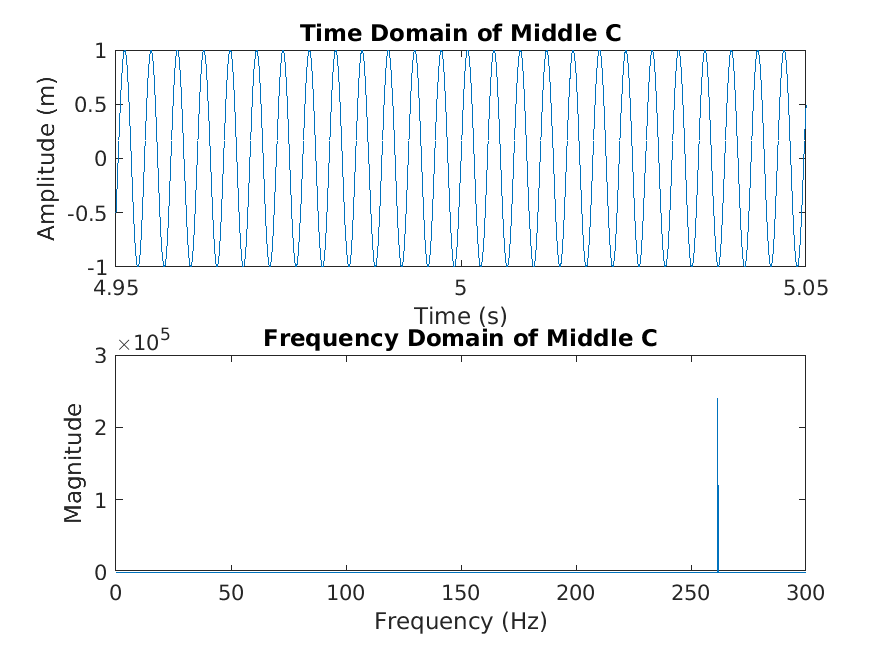
\includegraphics[width=\linewidth]{images/figure1.png}
  \caption{Time and Frequency domain of Middle C}
  \label{fig:middlec}
\end{figure}

\section{Time Domain}
\section{Frequency Domain}
\section{Frequency Filtering}
\section{Identifying Noise}
\section{Removing Noise}
\section{Extension}

\citep{gerardo_schneider}
\bibliographystyle{unsrt}
\bibliography{mybib}

\end{document}
